\documentclass{beamer}
\usepackage{ctex, hyperref}
\usepackage[T1]{fontenc}
\usepackage[most]{tcolorbox}
\usefonttheme{professionalfonts}
\usepackage{algorithm}
\usepackage{algpseudocode}
\usepackage{booktabs}
\usepackage{geometry} % 可选：调整页面边距，避免子图拥挤
% other packages
\usepackage{bm,latexsym,amsmath,xcolor,multicol,booktabs,calligra,tikz,subfigure,subcaption,caption}
\usepackage{graphicx,pstricks,listings,stackengine}
\usetikzlibrary{calc}
\captionsetup{font=small}

\author{你的姓名}
\title{这是你的标题}
\subtitle{副标题}
\institute{湘潭大学}
\date{\today}
\usepackage{NJUPT}

% defs
\def\cmd#1{\texttt{\color{red}\footnotesize $\backslash$#1}}
\def\env#1{\texttt{\color{blue}\footnotesize #1}}
\definecolor{deepblue}{rgb}{0,0,0.5}
\definecolor{deepred}{rgb}{0.6,0,0}
\definecolor{deepgreen}{rgb}{0,0.5,0}
\definecolor{halfgray}{gray}{0.55}
\definecolor{KuangNei}{RGB}{242,242,242}
\definecolor{BianKuang}{RGB}{71,93,79}
\lstset{
    basicstyle=\ttfamily\small,
    keywordstyle=\bfseries\color{deepblue},
    emphstyle=\ttfamily\color{deepred},    % Custom highlighting style
    stringstyle=\color{deepgreen},
    numbers=left,
    numberstyle=\small\color{halfgray},
    rulesepcolor=\color{red!20!green!20!blue!20},
    frame=shadowbox,
}


\begin{document}

\kaishu
\begin{frame}
    \titlepage
    \begin{figure}[htpb]
        \begin{center}
            
\includegraphics[width=0.2\linewidth]{pic/XTU.png}
        \end{center}
    \end{figure}
\end{frame}

\begin{frame}
    \tableofcontents[sectionstyle=show,subsectionstyle=show/shaded/hide,subsubsectionstyle=show/shaded/hide]
\end{frame}


\section{一个简单的例子}

\begin{frame}{一维Poisson方程}
\small
考虑一维Poisson方程的Dirichlet边值问题:
\begin{equation}
  \begin{cases}
-u''(x) = f(x), & x \in (0,1), \\
u(0) = u(1) = 0.
\end{cases}
\label{eq:1dimPD}
\end{equation}
\end{frame}

\begin{frame}
\small
关于$\{\varphi_j\}_{j=0}^{n}$的具体表达式形式很容易可以写出来,记$h_i=|x_{i-1}-x_i|$
$$
\varphi_0=
\begin{cases}
  \frac{x_1-x}{h_1},&x\in [x_0,x_1]\\
  0,&\text{其他}
\end{cases},
\varphi_n=
\begin{cases}
  0,&\text{其他}\\
  \frac{x-x_{n-1}}{h_n},&x\in [x_{n-1},x_n]
\end{cases}
$$
$$
\varphi_i=
\begin{cases}
  \frac{x-x_{i-1}}{h_i},&x\in [x_{i-1},x_i]\\
  \frac{x_{i+1}-x}{h_{i+1}},&x\in [x_i,x_{i+1}]\\
  0,&\text{其他}
\end{cases}
$$
\begin{center}
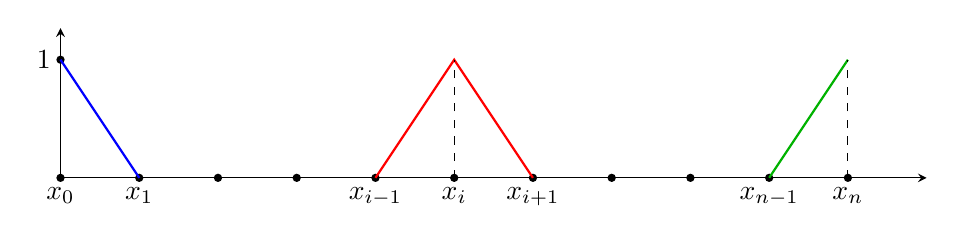
\begin{tikzpicture}[scale=10, >=stealth]

  % 绘制线段 [0,1]
  \draw[->] (0,0) -- (1.1,0);
  \draw[->] (0,0) -- (0,0.19);

  % 分成 10 段，共 11 个节点
  \foreach \i in {0,...,10} {
    \fill (\i/10,0) circle (0.15pt);
  }
  \fill (0,0.15) circle (0.15pt);
  % 下方标注 x_0, x_n
  \node[below] at (0,0) {$x_0$};
  \node[below] at (1,0) {$x_n$};
  \node[below] at (0.1,0) {$x_1$};
  \node[below] at (0.9,0) {$x_{n-1}$};
  \node[left] at (0,0.15) {$1$};

  % 第五、第六、第七个节点坐标
  \def\xA{0.4}  % x_{i-1}
  \def\xB{0.5}  % x_i
  \def\xC{0.6}  % x_{i+1}

  % 下方标注 x_{i-1}, x_i, x_{i+1}
  \node[below] at (\xA,0) {$x_{i-1}$};
  \node[below] at (\xB,0) {$x_i$};
  \node[below] at (\xC,0) {$x_{i+1}$};

  % 红色实线（屋顶）
  \draw[red, thick] (\xA,0) -- (\xB,0.15) -- (\xC,0);

  % 蓝色实线：f(x) = (x_i - x)/(x_i - x_{i-1})
  \draw[blue, thick] (0,0.15) -- (0.1,0);

  % 亮绿色实线：f(x) = (x - x_i)/(x_{i+1} - x_i)
  \draw[green!70!black, thick] (0.9,0) -- (1,0.15);
  \draw[dashed] (0.5,0) -- (0.5,0.15);
  \draw[dashed] (1,0) -- (1,0.15);

\end{tikzpicture}
\end{center}
\end{frame}


\begin{frame}
\small
在计算机上可以利用如下算法
\begin{algorithm}[H]
\caption{刚度矩阵的组装}
\begin{algorithmic}[1]
\State 初始化$n+1$阶零矩阵$K$
\For {$i=1,2,\cdots n$}
    \State 计算$2$阶局部刚度矩阵单元
    $$
    K^{(k)}=\frac{1}{h_k}
    \begin{bmatrix}
      1 & -1\\
      -1& 1 \\
    \end{bmatrix}
    $$
    \State $K_{ii}=K^{(k)}_{11}$
    \State $K_{i,i+1}=K^{(k)}_{12}$
    \State $K_{i+1,i}=K^{(k)}_{21}$
    \State $K_{i+1,i+1}= K^{(k)}_{22}$ 
\EndFor
\end{algorithmic}
\end{algorithm}
\end{frame}

\begin{frame}{边界条件}
\small
需要注意的是问题\eqref{eq:1dimPD}有边界条件$u(x_0)=u(x_n)=1$,因此刚度矩阵第一行以及最后一行应替换为
$$
(\underbrace{1,0,\cdots,0}_{n+1}),\quad (\underbrace{0,\cdots,0,1}_{n+1})
$$
载荷向量第一行与最后一行都是$0$
\end{frame}

\begin{frame}{数值算例}
\small
\centering

\begin{minipage}[b]{0.3\textwidth}
    \centering
    \captionof{subfigure}{$N=4$}
    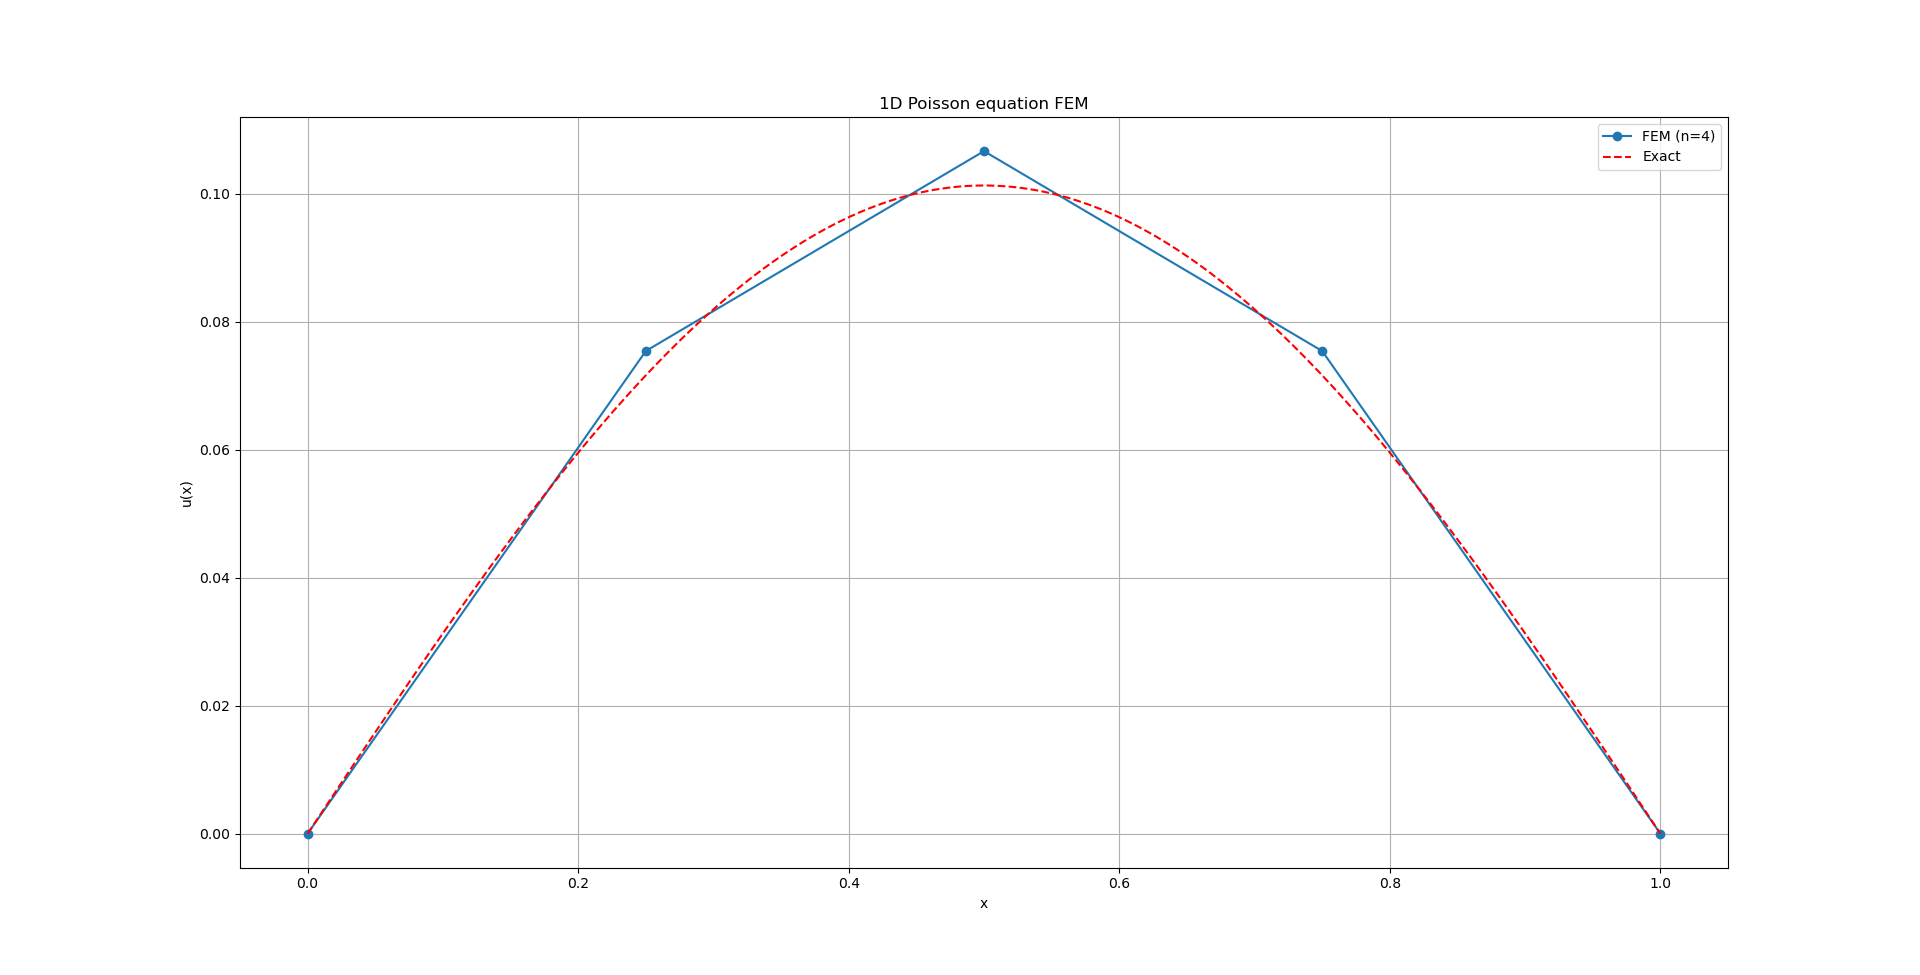
\includegraphics[width=\linewidth]{pic/n_4_global.png}
    
\end{minipage}
\hfill % 水平均匀间距
\begin{minipage}[b]{0.3\textwidth}
    \centering
    \captionof{subfigure}{$N=16$}
    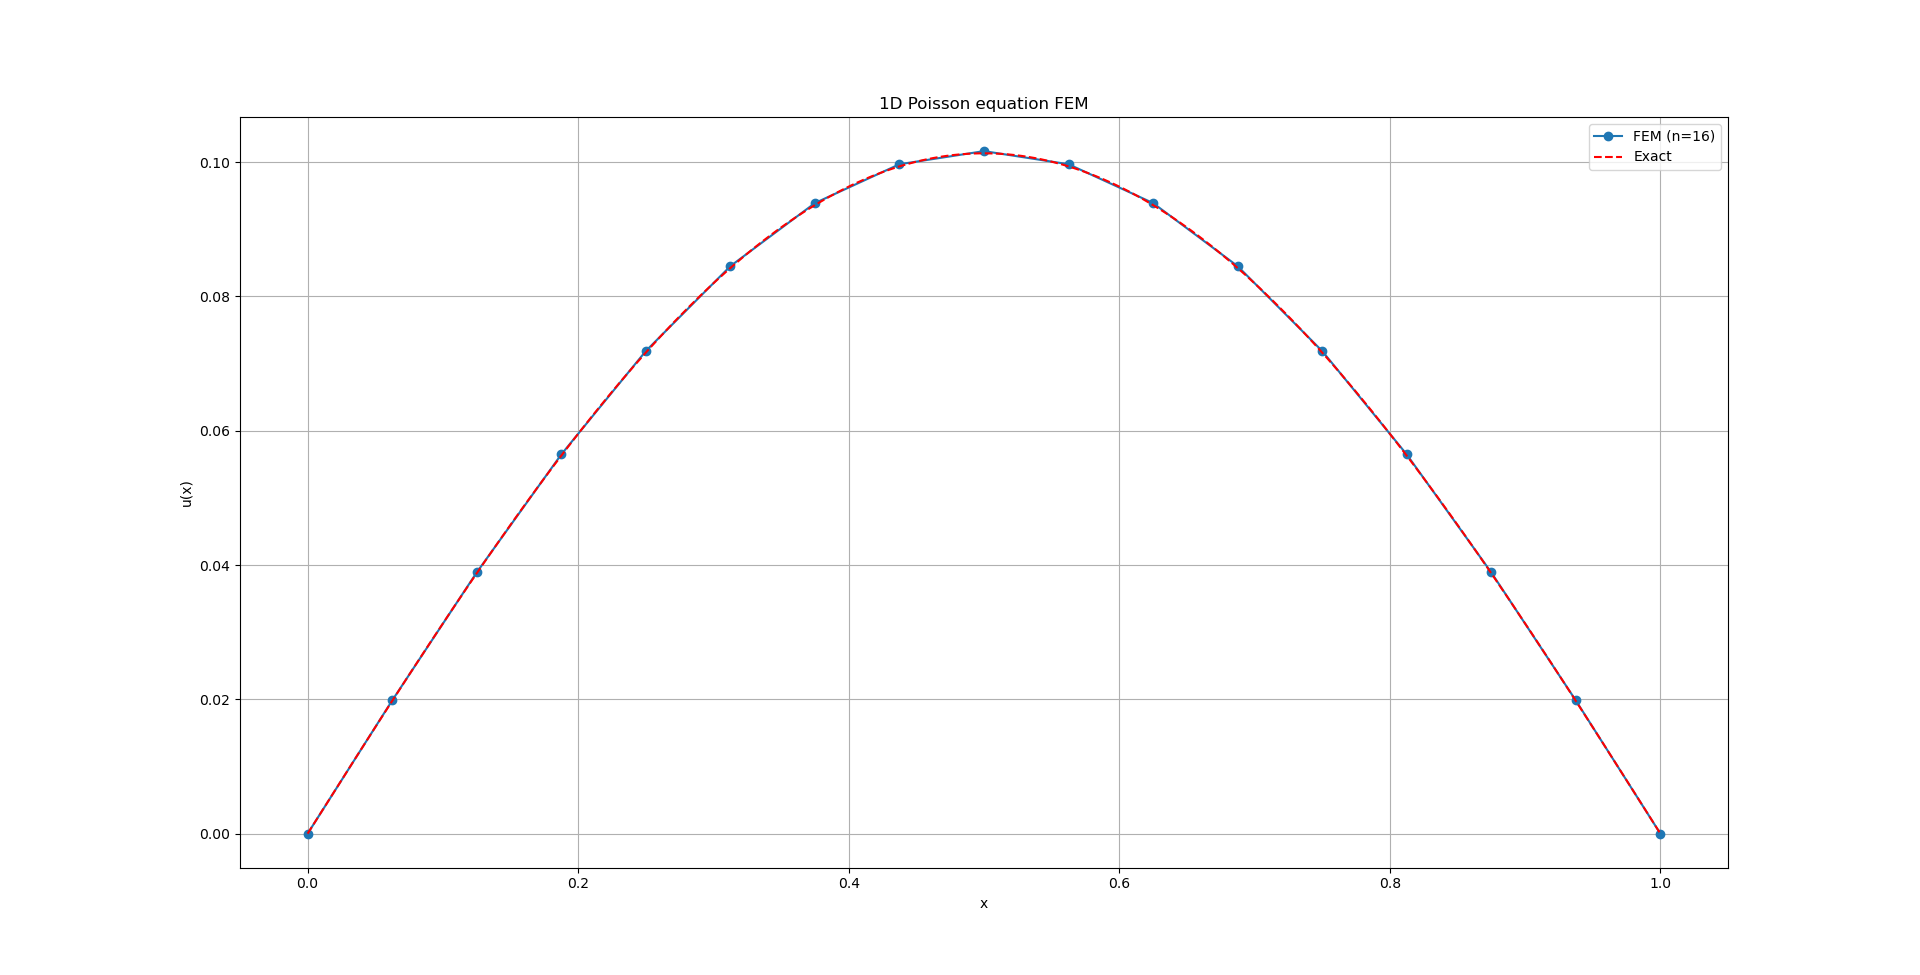
\includegraphics[width=\linewidth]{pic/n_16_global.png}
    
\end{minipage}
\hfill
\begin{minipage}[b]{0.3\textwidth}
    \centering
    \captionof{subfigure}{$N=128$}
    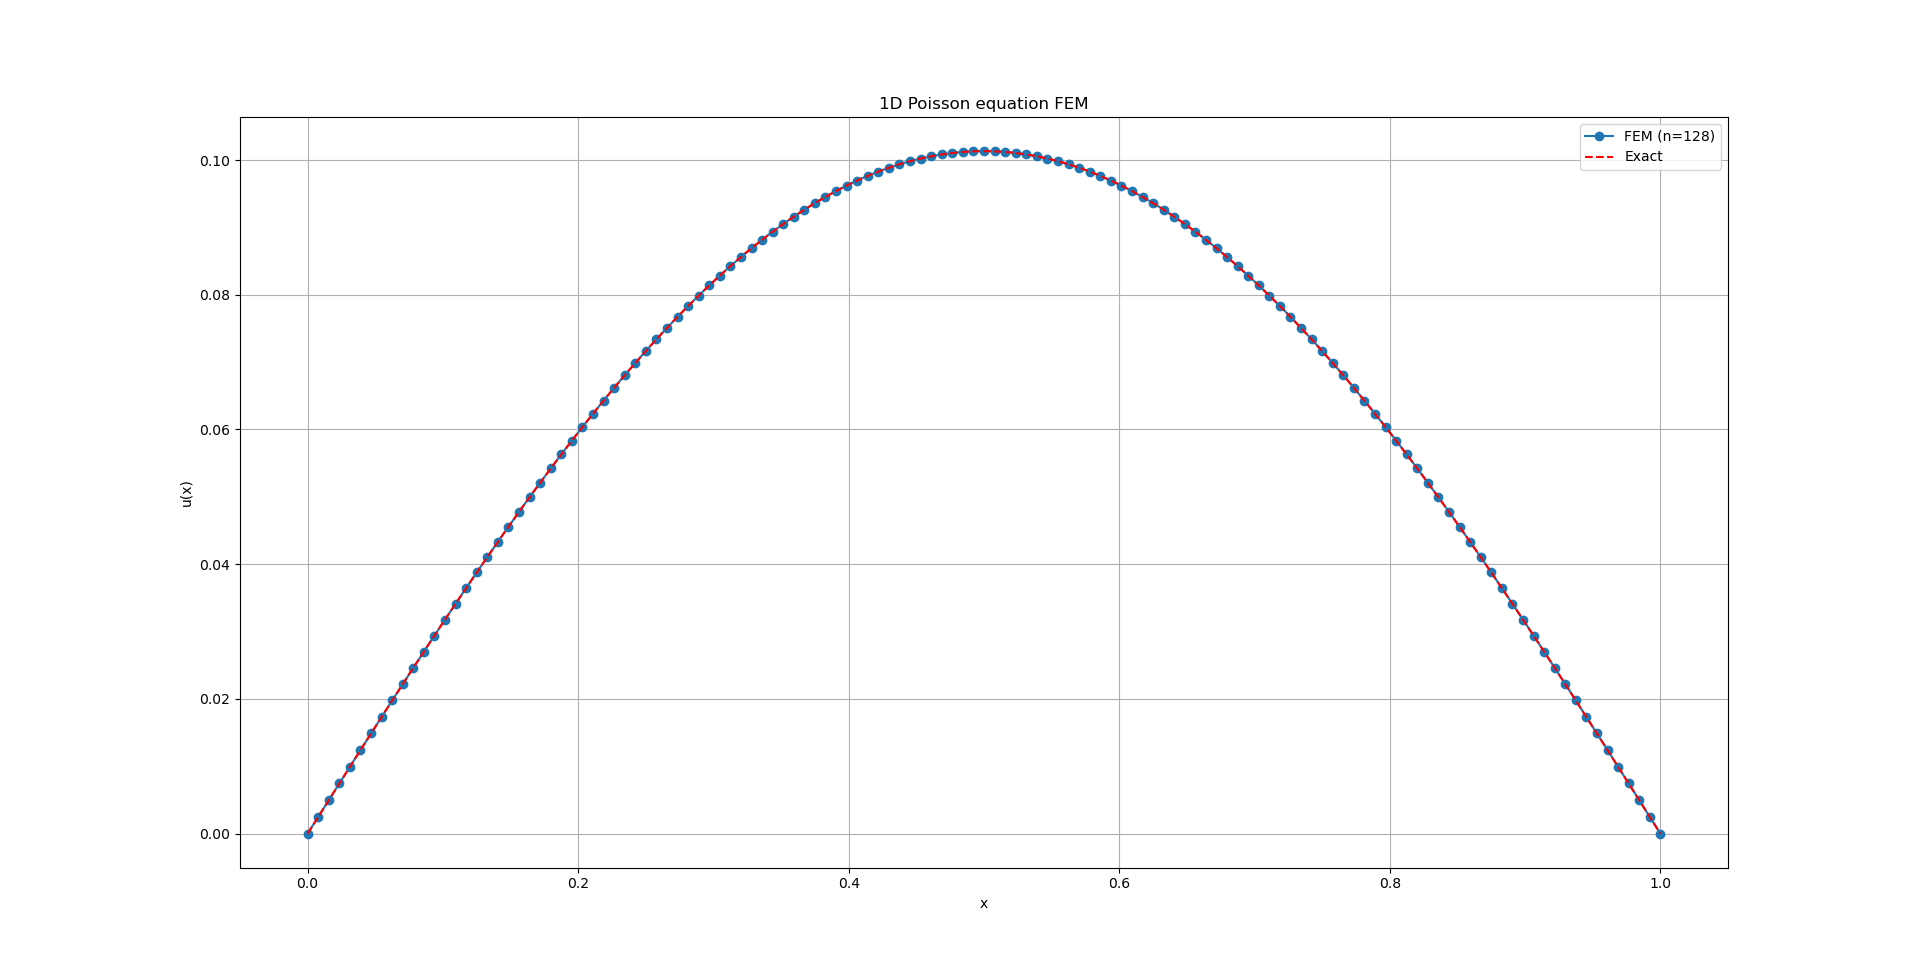
\includegraphics[width=\linewidth]{pic/n_128_global.png}
    
\end{minipage}

\vskip 0.3cm

\begin{minipage}[b]{0.3\textwidth}
    \centering
    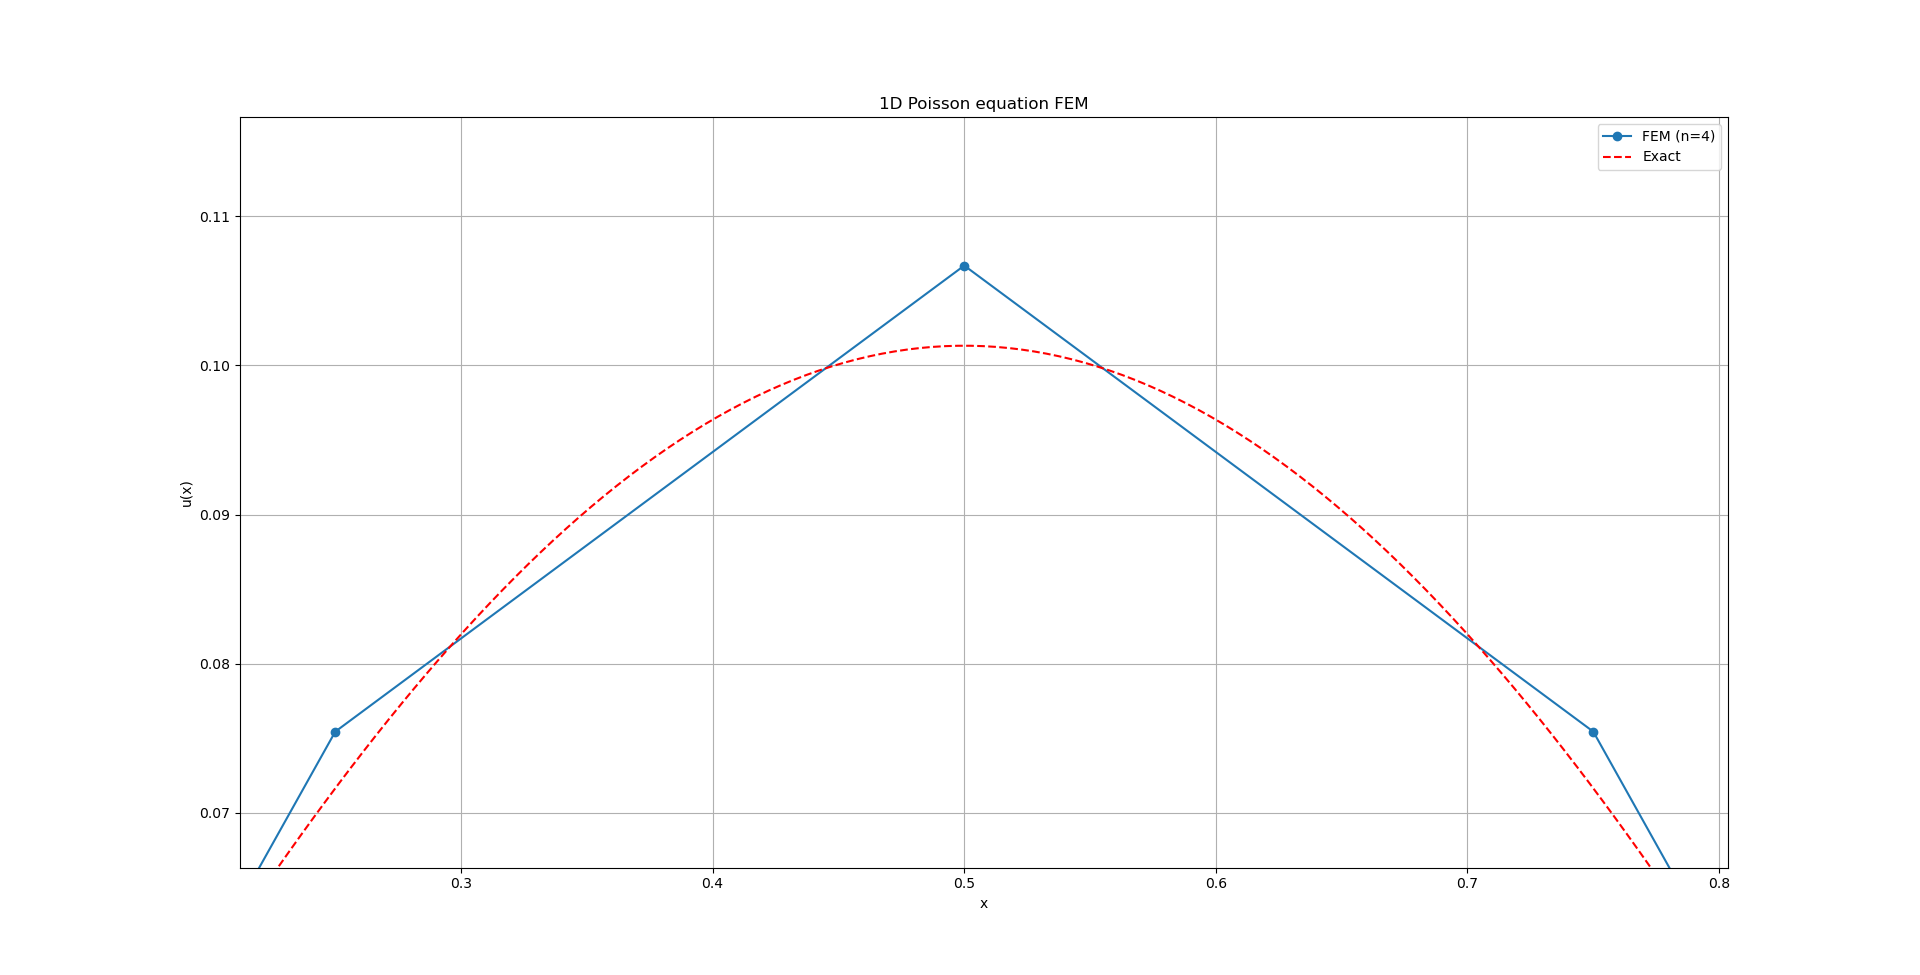
\includegraphics[width=\linewidth]{pic/n_4.png}
\end{minipage}
\hfill
\begin{minipage}[b]{0.3\textwidth}
    \centering
    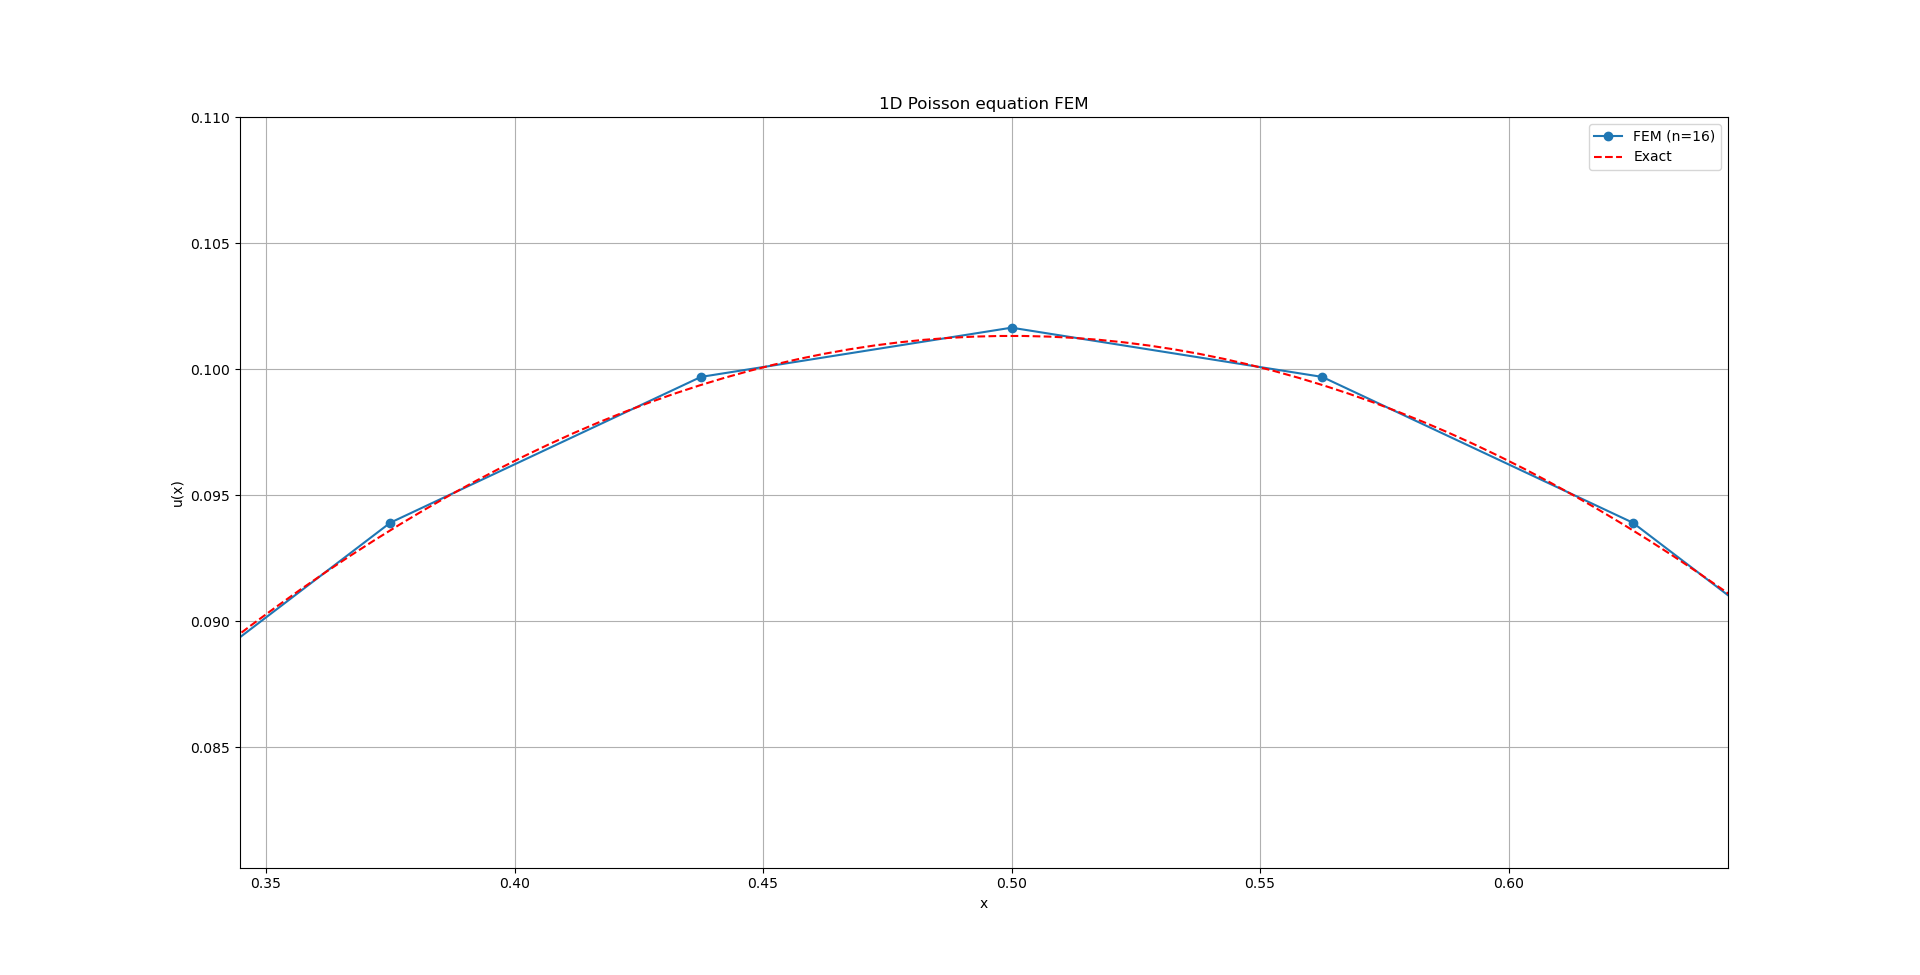
\includegraphics[width=\linewidth]{pic/n_16.png}
\end{minipage}
\hfill
\begin{minipage}[b]{0.3\textwidth}
    \centering
    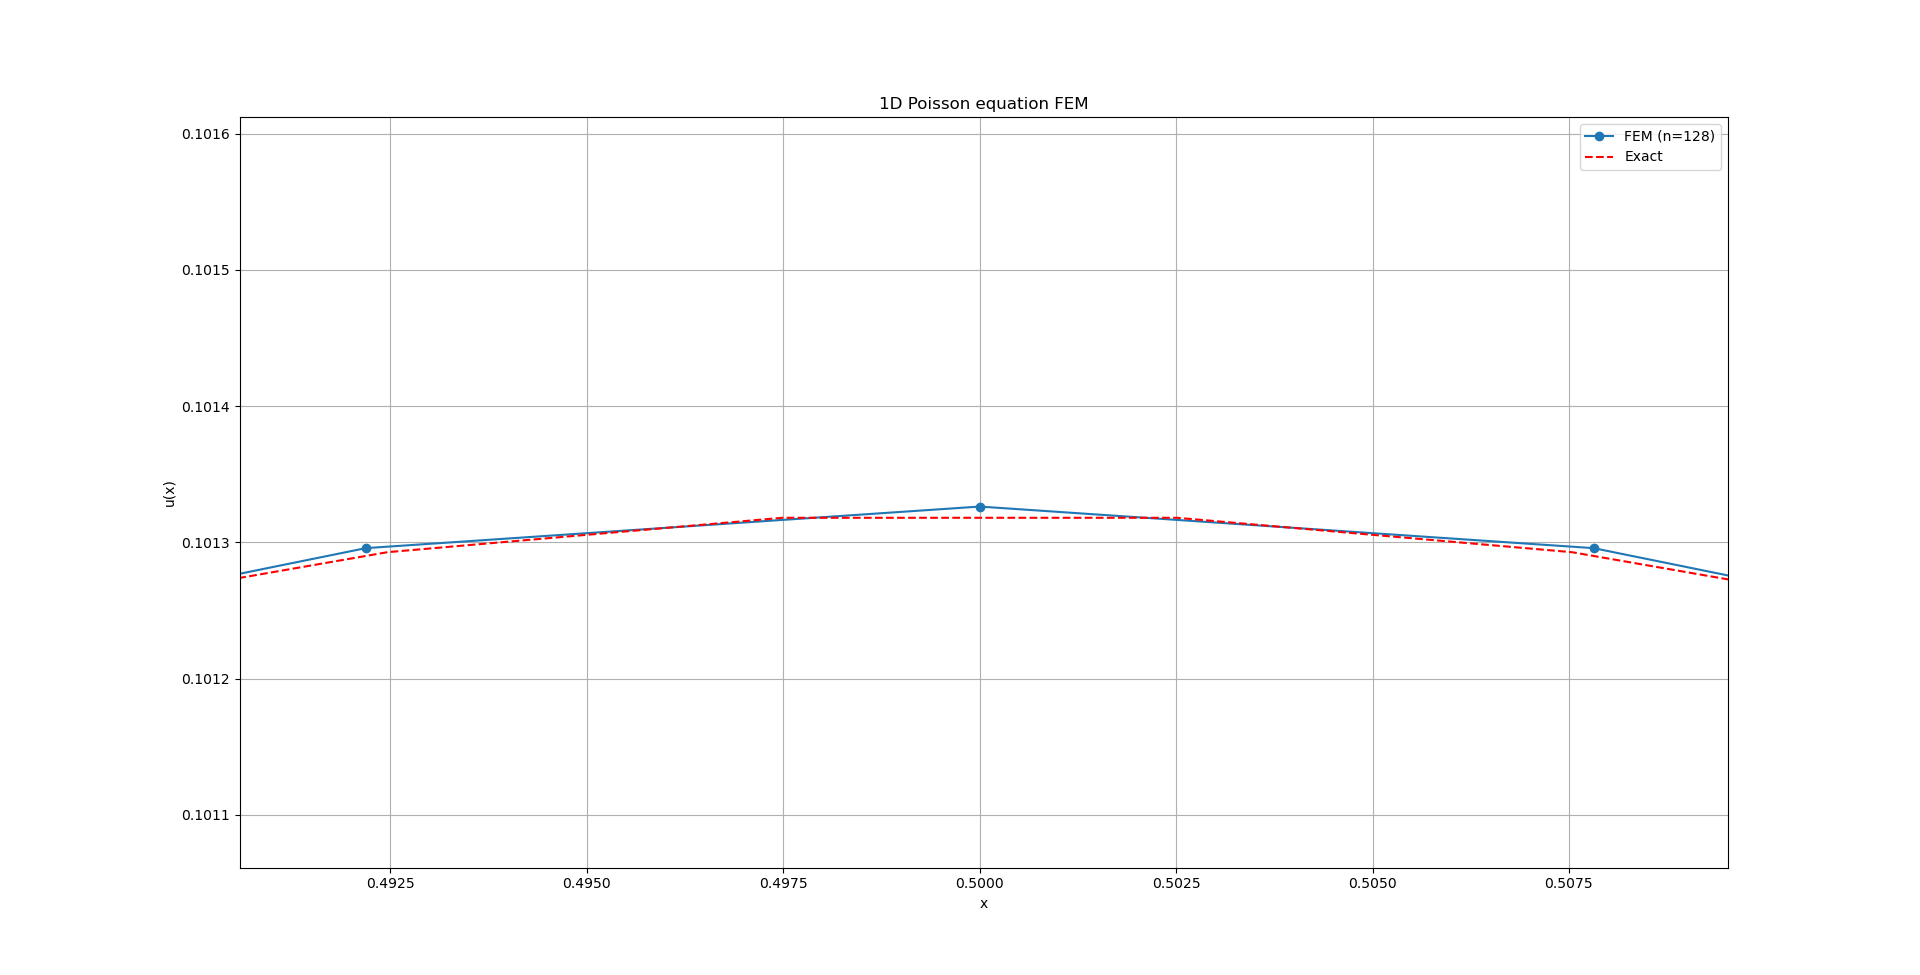
\includegraphics[width=\linewidth]{pic/n_128.png}
\end{minipage}
\end{frame}

\section{抽象有限元}
\subsection{抽象变分问题}
\begin{frame}{对双线性形式的要求}
\small
设$a(\cdot,\cdot)$是赋范线性空间$H$上的双线性形式.若存在常数$C>0$使得
$$
|a(v,w)|\leqslant C\|v\|_H\|w\|_H,\quad \forall v,w\in H
$$
我们称$a(\cdot,\cdot)$是有界的(连续的).若存在常数$\alpha >0$使得
$$
a(v,v)\geqslant \alpha \|v\|^2_H,\quad \forall v\in V\subset H
$$
我们称$a(\cdot,\cdot)$在$V\subset H$上强制.
\end{frame}

\begin{frame}{变分问题}
变分问题:设$H$为Hilbert空间,$V\subset H$为闭子空间,$a(\cdot,\cdot)$为$H$上的有界且在$V$上强制的双线性形式,那么非对称变分问题是指给定$F\in V'$,找到$u\in V$使得
\begin{equation}
    a(u,v)=\langle F,v\rangle,\quad \forall v\in V
    \label{eq:2.6.2}
\end{equation}
事实上,这个问题解的存在与唯一性可以通过下面的Lax-Milgram定理来保证
\end{frame}

\begin{frame}{Lax-Milgram}
\small
\begin{tcolorbox}[colback=white,colframe=njupt,title=\textbf{Lax-Milgram定理},sharpish corners]
    设$H$为Hilbert空间,$a(\cdot,\cdot)$为$H$上的有界且在$V$上强制的双线性形式,$F\in H'$,那么存在唯一的$u\in H$使得
    $$
    a(u,v)=\langle F,v\rangle,\quad \forall v\in H
    $$
\end{tcolorbox}
这个定理只是在无穷维空间上断言了解的存在唯一性.与刚开始的例子一样,我们需要寻找$V$的有限维子空间,在其上寻找近似解.
\end{frame}

\begin{frame}{有限维逼近}
\small
Galerkin逼近问题:给定一个有限维子空间$V_h\subset V$与$F\in V'$.寻找$u_h\in V_h$满足
\begin{equation}
    a(u_h,v)=\langle F,v\rangle,\quad \forall v\in V_h
    \label{eq:2.6.3}
\end{equation}
\end{frame}

\begin{frame}
\small
现在解决第二个问题:如何估计误差$u-u_h$?
\begin{tcolorbox}[colback=white,colframe=njupt,title=\textbf{Céa引理},sharpish corners]
    设$H$为Hilbert空间,$V\subset H$为闭子空间,$a(\cdot,\cdot)$为$H$上的有界且在$V$上强制的双线性形式,$F\in V'$.设$u\in V$是变分问题\eqref{eq:2.6.2}的解,$u_h\in V_h\subset V$是Galerkin逼近问题\eqref{eq:2.6.3}的解,则有
    $$
    \|u-u_h\|_V\leqslant \frac{C}{\alpha}\inf_{v\in V_h}\|u-v\|_V
    $$
    其中$C$是$a(\cdot,\cdot)$的有界常数,$\alpha$是$a(\cdot,\cdot)$在$V$上强制的常数.
\end{tcolorbox}
这个引理右边是$u$在$V_h$中的最佳近似误差,因此这个引理说明Galerkin逼近解$u_h$的误差不会比$u$在$V_h$中的最佳近似误差大多少倍.这就把误差估计问题转化为了如何构造有限维子空间$V_h$以及如何估计最佳近似误差的问题.\par
\end{frame}

\begin{frame}
\small
\textbf{定义}$^\clubsuit $:区域$\Omega$的一个划分,是有限个满足如下条件的单元域全体$\{K_i\}$:\par
1.$\operatorname{int} K_i\cap\operatorname{int}K_j=\emptyset,i\neq j$;\par
2.$\cup K_i=\overline{\Omega}$.\\[8pt]
\textbf{定义}$^\clubsuit $:设$\Omega$是一个有划分$\mathcal{T}$的区域.设划分中的每个单元$K$都定义了某种类型的形函数空间$\mathcal{P}$与节点变量集$\mathcal{N}$,使得$(K,\mathcal{P},\mathcal{N})$成为一个有限元.设$m$为节点变量所涉及的偏导数最高阶数.对于$f\in C^m(\overline{\Omega})$,其全局插值函数定义为
$$
\mathcal{I}_{\mathcal{T}}f|_{K_i}=\mathcal{I}_{K_i} f
$$
对所有的$K_i\in\mathcal{T}$.\par
\end{frame}

\begin{frame}
\small
对于一般情况,$k\geqslant 1$,$\mathcal{P}=\mathcal{P}_k$,$\mathcal{N}_k=\{N_i,i=1,\cdots,\frac{1}{2}(k+1)(k+2)\}$,我们按下面的规则选择节点位置:
$$
\begin{aligned}
  &3\text{个顶点}.\\
  &3(k-1)\text{个不同的边节点};\\
  &\frac{1}{2}(k-1)(k-2)\text{个单元内部节点}.
\end{aligned}
$$
\centering
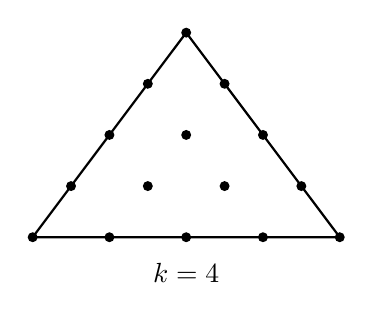
\begin{tikzpicture}[scale=3]
  % 等边三角形顶点（改这里就能匹配你原图的顶点）
  \def\Ax{0}     \def\Ay{0}
  \def\Bx{1.3}     \def\By{0}
  \def\Cx{0.65}   \def\Cy{0.86602540378} % sqrt(3)/2

  % 画三角形
  \draw[thick] (\Ax,\Ay) -- (\Bx,\By) -- (\Cx,\Cy) -- cycle;

  % k = 4
  \def\K{4}
  \foreach \i in {0,...,4}{
    \foreach \j in {0,...,4}{
      \pgfmathtruncatemacro{\t}{\K-\i-\j} % t = K - i - j
      \ifnum\t>-1 % 等价于 t >= 0
        % 计算笛卡尔坐标： x = (t*Ax + i*Bx + j*Cx)/K
        \pgfmathsetmacro{\x}{(\t*\Ax + \i*\Bx + \j*\Cx)/\K}
        \pgfmathsetmacro{\y}{(\t*\Ay + \i*\By + \j*\Cy)/\K}
        \fill (\x,\y) circle (0.6pt);
      \fi
    }
  }
  \node at (0.65,-0.15) {$k=4$};
\end{tikzpicture}
\hspace{1.8cm}
% ================= 右图 k=5 =================
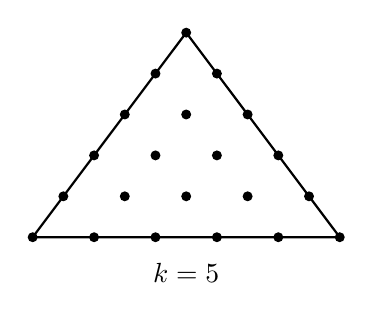
\begin{tikzpicture}[scale=3]
  % 和左图使用同样的顶点（保证两图视觉一致）
  \def\Ax{0}     \def\Ay{0}
  \def\Bx{1.3}     \def\By{0}
  \def\Cx{0.65}   \def\Cy{0.86602540378}

  \draw[thick] (\Ax,\Ay) -- (\Bx,\By) -- (\Cx,\Cy) -- cycle;

  % k = 5
  \def\K{5}
  \foreach \i in {0,...,5}{
    \foreach \j in {0,...,5}{
      \pgfmathtruncatemacro{\t}{\K-\i-\j}
      \ifnum\t>-1
        \pgfmathsetmacro{\x}{(\t*\Ax + \i*\Bx + \j*\Cx)/\K}
        \pgfmathsetmacro{\y}{(\t*\Ay + \i*\By + \j*\Cy)/\K}
        \fill (\x,\y) circle (0.6pt);
      \fi
    }
  }
  \node at (0.65,-0.15) {$k=5$};
\end{tikzpicture}
\end{frame}


\section{stokes方程}

\begin{frame}{致谢}
\begin{center}
    感谢各位聆听！\\[8pt]
\end{center}
\end{frame}

\end{document}